\subsection{Modelos de Aprendizado de M\'aquina Supervisionados}\label{subsec:reg}

Os modelos regressivos para séries temporais têm sido amplamente reconhecidos e utilizados na literatura atual, especialmente aqueles baseados em métodos de gradiente. Esses modelos, incluindo a regressão linear simples, têm se destacado como uma escolha popular em competições de séries temporais em todo o mundo.

Esses modelos são valorizados por sua capacidade de capturar relações complexas e não lineares nos dados, permitindo previsões mais precisas e eficientes. Sua popularidade reflete o reconhecimento da eficácia desses modelos em abordar uma ampla gama de problemas de previsão de séries temporais em diferentes áreas de estudo.

A abordagem regressiva, combinada com técnicas de otimização baseadas em gradiente, tem se mostrado particularmente eficaz na obtenção de resultados de alta qualidade. Esses modelos são capazes de aprender a partir dos dados históricos e ajustar seus parâmetros de forma iterativa, otimizando assim o desempenho da previsão.

Com a crescente disponibilidade de dados e avanços na área de aprendizado de máquina, espera-se que os modelos regressivos para séries temporais continuem a evoluir e desempenhar um papel importante na análise e previsão de dados temporais em diversas aplicações.

\subsubsection{Prophet}


O Prophet é um modelo de previsão de séries temporais desenvolvido pelo Facebook. Foi projetado para simplificar a previsão de séries temporais comuns que apresentam padrões sazonais, tendências e feriados. O Prophet é especialmente útil para usuários que desejam realizar previsões precisas sem requerer um profundo conhecimento em estatística ou aprendizado de máquina.

O modelo se baseia em uma abordagem aditiva que desagrega a série temporal em vários componentes individuais, como tendência de longo prazo, sazonalidade semanal e anual, e efeitos de feriados. Esses componentes são combinados para formar uma previsão geral.
A equação básica do modelo Prophet pode ser representada da seguinte forma:

\begin{eqnarray}
	 y(t) &=& g(t) + s(t) + h(t) + \varepsilon_t 
\end{eqnarray}

\noindent onde, \( y(t) \) é o valor da série temporal no tempo \( t \), que se deseja prever. \( g(t) \) representa a tendência de longo prazo da série. \( s(t) \) representa os componentes sazonais, que podem incluir padrões semanais e anuais. \( h(t) \) é a representação dos efeitos de feriados ou eventos especiais. \( \varepsilon_t \) é o erro aleatório ou ruído na previsão.


O modelo Prophet ajusta esses componentes aos dados históricos de séries temporais para criar uma previsão futura. Ele utiliza um procedimento de ajuste automático para estimar os parâmetros desses componentes com base nos dados fornecidos. A abordagem aditiva do Prophet permite que os padrões sazonais, tendências e feriados sejam capturados separadamente e, em seguida, somados para gerar uma previsão global \cite{2-s2.0-85092514286}.

Lembrando que essa é uma perspectiva simplificada da equação do Prophet. O modelo em sua totalidade incorpora uma gama de ajustes e considerações destinados a aprimorar a precisão das previsões, incluindo o tratamento de incertezas, a seleção automática de sazonalidades relevantes e outras otimizações. 



\subsubsection{Correla\c c \~ao de Pearson}

Nos modelos de aprendizado de máquina supervisionados, é feita uma tentativa de identificar as relações existentes entre diferentes variáveis \cite{korstanje2021}:

Variável de destino: a variável que tenta prever.
Variáveis explicativas: Variáveis que ajudam a prever o alvo variável


Para realizar previsões, é importante que se compreenda quais tipos de variáveis explicativas podem ser utilizadas. Neste exemplo, a variável \textbf{Pressão de Sucção (PT01SU)} será considerada como a variável $x$, enquanto a variável \textbf{Nível do Reservatório (Câmara 1) LT01} será considerada como a variável $y$. O coeficiente de correlação indica a relação entre o eixo $x$ e $y$, como expresso pela seguinte fórmula.
A equação do coeficiente de correlação de Pearson é dada por:

\begin{equation}
	r=\frac{\sum\left(x_i-\bar{x}\right)\left(y_i-\bar{y}\right)}{\sqrt{\left(\sum\left(x_i-\bar{x}\right)^2\right)\left(\sum\left(y_i-\bar{y}\right)^2\right)}}
\end{equation}

\noindent onde $x_i$ e $y_i$ representam os valores das variáveis $X$ e $Y$, respectivamente. $\bar{x}$ e $\bar{y}$ são as médias dos valores $x_i$ e $y_i$. O coeficiente de correlação de Pearson mede a força e a direção da relação linear entre as variáveis $X$ e $Y$. Valores próximos a 1 indicam uma correlação positiva forte, valores próximos a -1 indicam uma correlação negativa forte, e valores próximos a 0 indicam uma ausência de correlação entre as variáveis.



\subsubsection{Regress\~ao Linear (LR)}

A regressão linear é definida da seguinte forma:

\begin{equation}
	y = \beta_0 + \beta_1 x_1 + \cdots + \beta_p x_p + \varepsilon \label{eq:lr}
\end{equation}

\noindent onde há $p$ variáveis explicativas, denotadas por $x$. Existe uma variável alvo, denotada por $y$. O valor de $y$ é calculado como uma constante $\beta_0$, somada aos valores das variáveis $x$ multiplicados por seus coeficientes $\beta_1$ a $\beta_p$.


Para utilizar a regressão linear, é necessário estimar os coeficientes (betas) com base em um conjunto de dados de treinamento. Esses coeficientes podem ser estimados por meio da seguinte fórmula, expressa em notação matricial:

\begin{eqnarray}
	\hat{\beta}&=&\left(X^T X\right)^{-1} X^T y\label{eq:ols}
\end{eqnarray}

\noindent a equação \eqref{eq:ols} mencionada, conhecida como \textbf{OLS} (método dos mínimos quadrados ordinários), é amplamente utilizada na regressão linear \citeonline{korstanje2021}. Esse método é conhecido por ser rápido de ajustar, pois requer apenas cálculos matriciais para estimar os coeficientes $\beta$. No entanto, ele é mais adequado para processos lineares e pode ser menos adequado para modelos mais complexos que envolvam relações não-lineares. Portanto, é importante considerar suas limitações ao aplicar a regressão linear em contextos mais complexos.


\subsubsection{Regressor de \'Arvore de Decis\~ao }


Uma árvore de decisão (do ingl\^es \textit{Decision Tree Regressor}) é um dos algoritmos de aprendizado de máquina mais usados para resolver problemas de regressão e classificação. Como o nome sugere, o algoritmo usa um modelo de decisões semelhante a uma árvore para prever o valor de destino (regressão) ou prever a classe de destino (classificação). Antes de mergulhar em como as árvores de decisão funcionam, primeiro, vamos nos familiarizar com as terminologias básicas de uma árvore de decisão \cite{decision}:

Na Figura \ref{fig:decison} trás \textbf{Nó raiz} isso representa o nó mais alto da árvore que representa todos os pontos de dados.
\textbf{Divisão} refere-se à divisão de um nó em dois ou mais sub-nós.
\textbf{Nó de decisão} eles são os nós que são divididos em sub-nós, ou seja, esse nó que é dividido é chamado de nó de decisão.
\textbf{Nó Folha / Terminal} os nós que não se dividem são chamados de nós Folha ou Terminal. Esses nós são geralmente o resultado final da árvore.
\textbf{Ramo / Subárvore} uma subseção de toda a árvore é chamada de galho ou subárvore.
\textbf{Nó pai e filho} um nó, que é dividido em sub-nós é chamado de um nó pai de sub-nós, enquanto sub-nós são o filho do nó pai. Na figura acima, o nó de decisão é o pai dos nós terminais (filho).
\textbf{Poda} a remoção de sub-nós de um nó de decisão é chamada de poda. A poda costuma ser feita em árvores de decisão para evitar o \textit{overfitting}  \cite{decision}.

\begin{figure}[H]
	\centering
	\caption{Fluxograma da árvore de decisão}
	\label{fig:decison}
	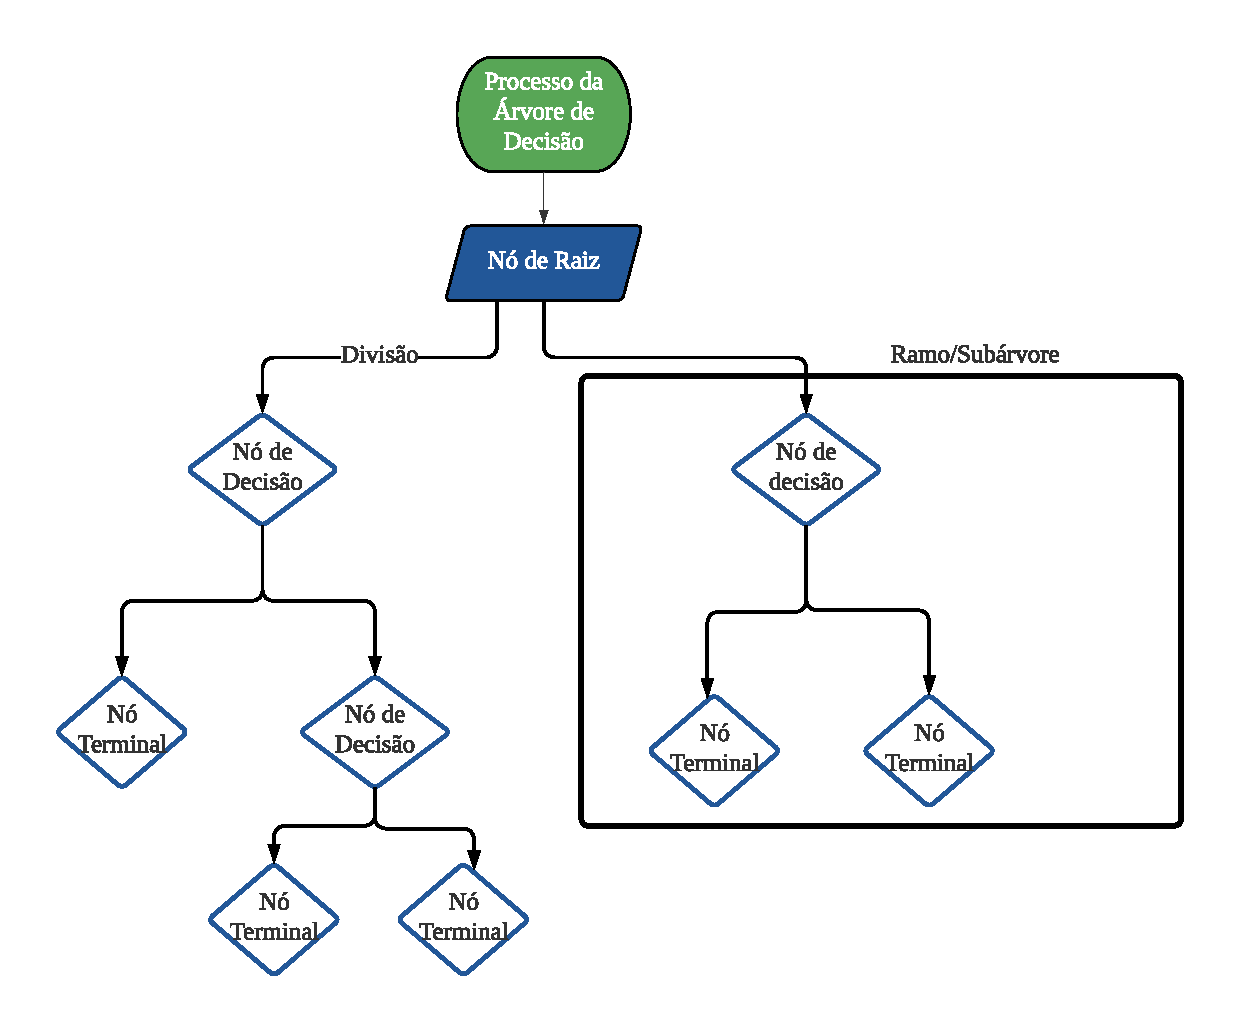
\includegraphics[width=0.9\linewidth]{Modelos/Figuras/decison}
	
	\fonte{Adaptado de \citeonline{decision}}
\end{figure}



\noindent\textbf{Vantagens}:


De fácil intuição e interpretação, já que podemos facilmente visualizá-las (quando não são muito profundas).
Requerem pouco esforço na preparação dos dados, métodos baseados em árvores normalmente não requerem normalização dos dados, codificação e variáveis fictício. Além disso, conseguem lidar com valores faltantes, categóricos e numéricos.
Complexidade logarítmica na etapa de predição.
São capazes de lidar com problemas com múltiplos rótulos.
Relações não-lineares entre parâmetros não afetam o desempenho da árvore \cite{remigio2023arvores}.


\noindent\textbf{Desvantagens}:

Árvore crescida até sua profundidade máxima pode decorar o conjunto de treino (\textit{overfitting}), o que pode degradar seu poder preditivo quando aplicado a novos dados. Isso pode ser mitigado “podando” a árvore de decisão ao atribuir uma profundidade máxima ou uma quantidade máxima de folhas.
São modelos instáveis (alta variância), pequenas variações nos dados de treino podem resultar em árvores completamente distintas. Isso pode ser evitado ao treinarmos várias árvores distintas e agregar suas predições.
O algoritmo de construção da árvore de decisão é ganancioso, ou seja, não garante a construção da melhor estrutura para o dados de treino em questão. Esse problema também pode ser mitigado ao treinarmos várias árvores distintas e agregar suas predições \cite{remigio2023arvores}.


\textbf{Aplicação}:

No contexto da previsão da demanda de água na Sanepar em Curitiba, é crucial considerar elementos como as flutuações climáticas, eventos particulares na cidade (como feriados) e padrões históricos de consumo. É fundamental reconhecer a eventualidade de que a árvore de decisão possa adquirir maior complexidade devido à diversidade de fatores que impactam a demanda de água.

Na Figura \ref{fig:arvore-de-decisao}, é demonstrado como o processo é representado por meio de uma árvore de decisão, em relação ao mapa mental.

\begin{figure}[H]
	\centering
	\caption{Árvore de decisão mapa mental}
	\label{fig:arvore-de-decisao}
	\includegraphics[width=0.7\linewidth]{"Apendices/Figuras/modelagem-24h/Árvore de decisão"}
	
	\fonte{Elaboração própria}
\end{figure}



\subsubsection{Floresta Aleat\'oria } \label{subsubsec:rf}

Pode-se observar que ter exatamente a mesma árvore de decisão repetidas vezes não adiciona valor significativo em comparação a usar essa mesma árvore de decisão apenas uma vez. Em modelos de conjunto, cada modelo individual deve ser ligeiramente diferente dos demais. Existem dois métodos amplamente reconhecidos para criar conjuntos: o ensacamento (\textit{bagging}) e o reforço (\textit{boosting}). A floresta aleatória (do inglês \textit{Random Forest}) utiliza o ensacamento para criar um conjunto de árvores de decisão, onde cada árvore é construída com uma amostra aleatória do conjunto de dados original. Isso garante que as árvores sejam distintas e diversificadas, contribuindo para a robustez e eficácia do modelo.



Cada árvore em um modelo de Floresta Aleatória de Regressão (RFR) é construída por meio de um algoritmo de aprendizado individual que divide o conjunto de variáveis de entrada em subconjuntos, com base em um teste de valor de atributo, como o coeficiente de Gini. Ao contrário das árvores de decisão clássicas, as árvores de RFR são construídas sem poda e selecionam aleatoriamente um subconjunto de variáveis de entrada em cada nó. Atualmente, o número de variáveis utilizadas para dividir um nó em uma RFR (denotado por $m$) corresponde à raiz quadrada do número total de variáveis de entrada. Essa abordagem ajuda a aumentar a diversidade das árvores e aprimorar o desempenho do modelo \cite{Pelletier2016156}.

\begin{figure}[!htb]
	\centering
	\caption{Esquema da Floresta Aleatória}
	\label{fig:rf}
	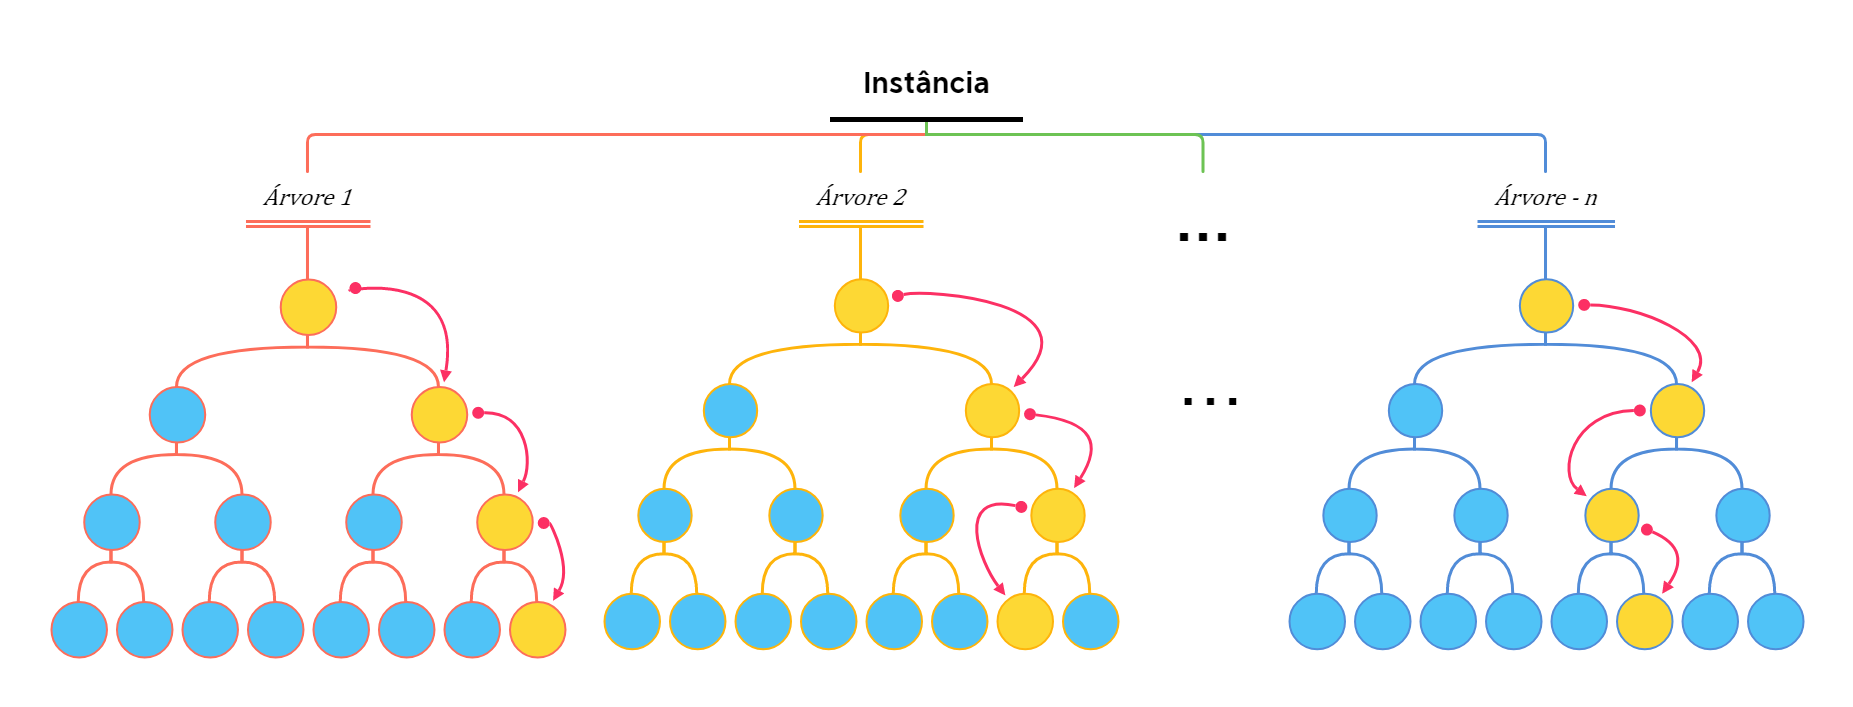
\includegraphics[width=1\linewidth]{Modelos/Figuras/RF}
	
	\fonte{Elaboração própria}
\end{figure}


\subsubsection{Gradient Boosting (como XGBoost, LightGBM)}\label{subsubsec:lgbxgb}

O aumento de gradiente (do inglês\textit{gradient boosting}) é um método que combina vários modelos de árvore de decisão para realizar previsões. Cada uma dessas árvores de decisão é única, pois a diversidade é um elemento importante nesse processo. A diversidade é alcançada através de um processo chamado boosting, que é uma abordagem iterativa. O boosting adiciona modelos fracos ao conjunto de forma inteligente, dando mais peso aos pontos de dados que ainda não foram bem previstos. 

O processo de boosting melhora o conjunto ao focar nas partes dos dados que ainda não são compreendidas. A Figura \ref{fig:xgboost} apresenta uma visão esquemática desse processo. À medida que novos modelos fracos são adicionados, todos os modelos fracos intermediários são mantidos. O modelo final é uma combinação de todos esses modelos fracos, resultando em um ensemble que oferece uma melhor capacidade de previsão do que um único modelo.

O boosting é apenas um dos métodos de ensemble utilizados em conjunto com o bagging. O bagging também é um método que utiliza múltiplos modelos de árvore de decisão, porém, em vez de adicionar os modelos de forma iterativa, cada modelo é treinado independentemente em subconjuntos aleatórios dos dados de treinamento. Ambos os métodos, boosting e bagging, têm como objetivo melhorar o desempenho do modelo combinando as previsões de múltiplos modelos individuais.


\begin{figure}[H]
	\centering
	\caption{Impulsionando gradiente com XGBoost e LightGBM}
	\label{fig:xgboos}
	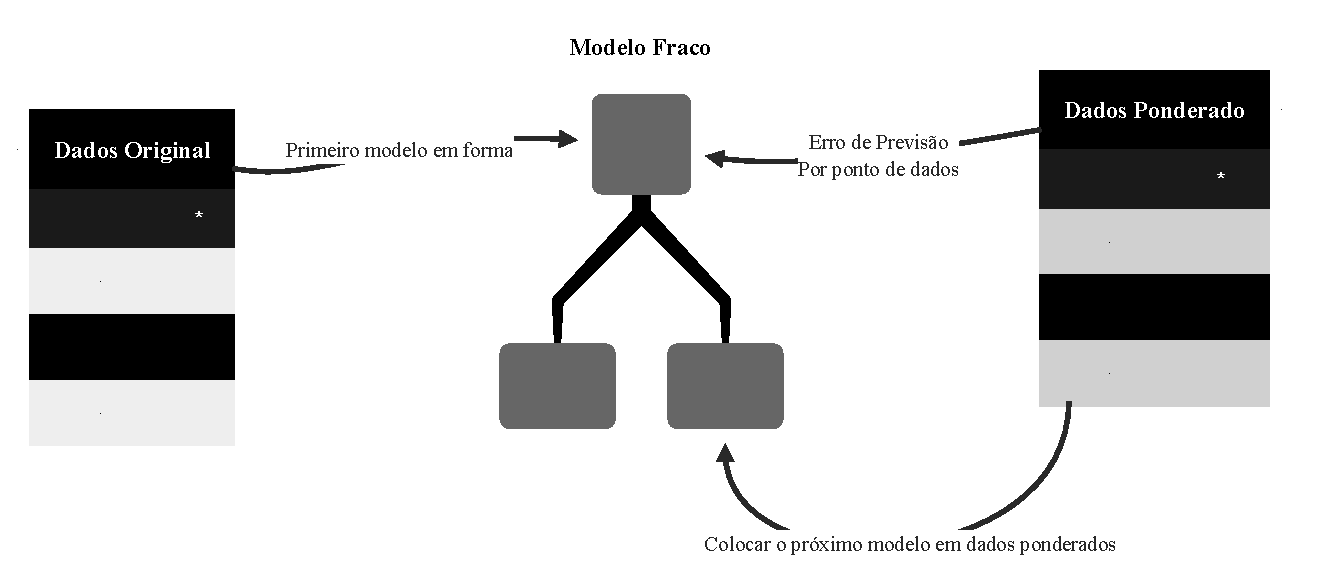
\includegraphics[width=1\linewidth]{Modelos/Figuras/xgboos}
	
	\fonte{Adaptação de \citeonline{korstanje2021}}
\end{figure}



\subsubsection{Gradiente de Boosting (Refor\c co)} \label{subsubsec:boosting}

O processo iterativo utilizado no aumento de gradiente, como descrito por \citeonline{korstanje2021}, recebe esse nome por um motivo. O termo ``gradiente'' refere-se a um campo vetorial de derivadas parciais que apontam na direção da inclinação mais acentuada. De forma simplificada, podemos pensar nos gradientes como as inclinações das estradas: quanto maior a inclinação, mais íngreme a colina. Para calcular os gradientes, são realizadas derivadas ou derivadas parciais de uma função.

No aumento de gradiente, ao adicionar árvores adicionais ao modelo, o objetivo é incorporar uma árvore que explique melhor a variação que ainda não foi explicada pelas árvores anteriores. Dessa forma, a nova árvore tem como objetivo ajustar-se aos erros ou resíduos deixados pelas árvores anteriores.

\begin{equation}
	y-\hat{y} \label{eq:xb}
\end{equation}

\noindent a equação \eqref{eq:xb} pode ser reescrita como a derivada parcial negativa da função de perda em relação às previsões $\hat{y}$:

\begin{equation}
	y-\hat{y} = -\dfrac{\partial L}{\partial \hat{y}} \label{eq:xb2}
\end{equation}

\noindent isso é definido como o objetivo da nova árvore a ser adicionada no modelo de aumento de gradiente, garantindo que ela explique a máxima quantidade de variação adicional no modelo geral. Essa é a razão pela qual o modelo é chamado de ``aumento de gradiente'' (do inglês ``\textit{gradient boosting}''). O processo utiliza o gradiente da função de perda para guiar a adição de novas árvores, buscando minimizar o erro e melhorar a capacidade do modelo em explicar a variação nos dados.

\noindent\textbf{Algoritmos de boosting de gradiente}

O \textbf{XGBoost} é um dos algoritmos de aprendizado de máquina mais utilizados. É uma forma rápida de obter bom desempenho. Devido à sua facilidade de uso e alto desempenho, é frequentemente o primeiro algoritmo escolhido por muitos profissionais de aprendizado de máquina.

O \textbf{LightGBM} é outro algoritmo de aumento de gradiente que é importante conhecer. Atualmente, é um pouco menos difundido que o XGBoost, mas está ganhando popularidade rapidamente. A vantagem esperada do LightGBM em relação ao XGBoost é um ganho de velocidade e uma utilização mais eficiente de memória.


\noindent\textbf{A diferen\c ca entre XGBoost e LightGBM}

Uma diferença fundamental reside na maneira como esses algoritmos identificam as melhores divisões entre os nós das árvores de decisão individuais. É crucial lembrar que uma divisão em uma árvore de decisão ocorre quando a árvore precisa encontrar a separação que mais melhora o desempenho do modelo.
A abordagem intuitiva e simples para encontrar a melhor divisão é iterar por todas as possibilidades e selecionar a melhor. No entanto, essa abordagem é computacionalmente custosa, e algoritmos mais recentes apresentam alternativas mais eficientes.

Uma alternativa proposta pelo XGBoost é a segmentação baseada em histograma. Nesse caso, em vez de iterar por todas as partições possíveis, o modelo constrói um histograma para cada variável e utiliza-os para encontrar a melhor divisão geral entre as variáveis.
O LightGBM, desenvolvido pela Microsoft, adota uma abordagem mais eficiente para a definição das divisões. Essa abordagem é conhecida como amostragem GOSS (unilateral baseada em gradiente). O GOSS calcula o gradiente para cada ponto de dados e utiliza-o para filtrar os pontos de dados com gradientes baixos. Afinal, os pontos de dados com gradientes baixos já são bem compreendidos, enquanto aqueles com gradientes altos precisam ser melhor aprendidos.

O LightGBM também utiliza uma abordagem chamada Exclusive EFB (do inglês \textit{Feature Bundling}), que acelera a seleção de muitas variáveis correlacionadas. Outra diferença é que o modelo LightGBM é adequado para o crescimento de folhas (do inglês \textit{leaf-wise growth}), enquanto o XGBoost cultiva as árvores em níveis. Essa diferença pode ser visualizada na Figura \ref{fig:xgboost}.
Essa diferença teoricamente favorece o LightGBM em termos de precisão, mas também apresenta um maior risco de sobre-ajuste (do inglês \textit{overfitting}) quando há poucos dados disponíveis. Portanto, é importante que a pessoa considere essas distinções ao escolher entre os dois algoritmos de aumento de gradiente.

Na Figura \ref{fig:xgboost}, é possível visualizar como cada modelo é ajustado durante o processo de crescimento de árvore em folhas e em níveis. Essa representação gráfica oferece uma compreensão visual das diferenças entre os dois métodos.

\begin{figure}[H]
	\centering
	\caption{Compara-se o crescimento em folha com o crescimento em nível}
	\label{fig:xgboost}
	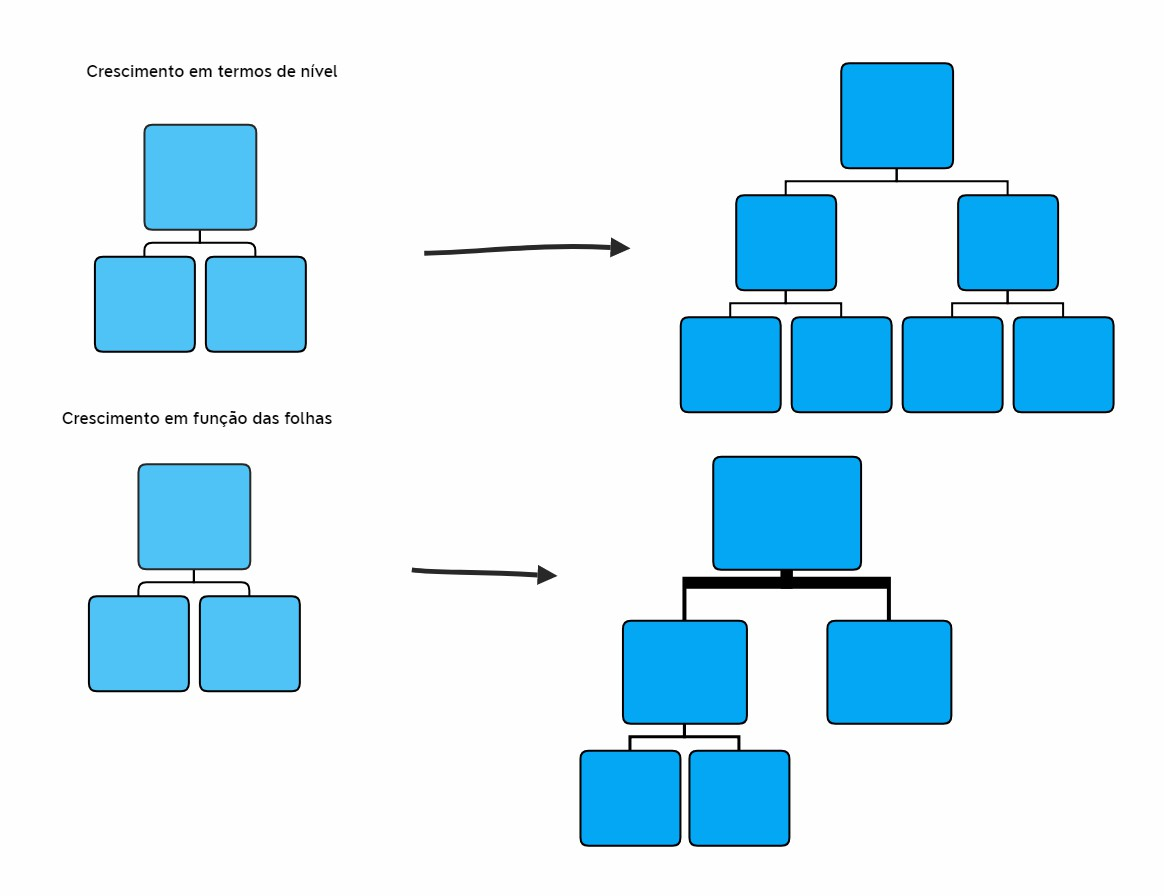
\includegraphics[width=0.7\linewidth]{Modelos/Figuras/xgboost}
	
	\fonte{Adaptação de \citeonline{korstanje2021}}
\end{figure}


No crescimento de árvore em folhas, como no LightGBM, novas folhas são adicionadas à árvore de forma iterativa, visando maximizar a redução do erro de treinamento. Isso significa que as árvores são expandidas adicionando folhas, uma a uma, até que o critério de parada seja alcançado.
Por outro lado, no crescimento em níveis, como no XGBoost, as árvores são expandidas em profundidade de forma simultânea em todos os níveis. Ou seja, em cada nível, todas as folhas são expandidas ao mesmo tempo, resultando em um crescimento mais uniforme da árvore.

Essa distinção no modo de crescimento das árvores pode afetar o comportamento e o desempenho do modelo. Portanto, compreender essa diferença é importante ao escolher entre esses algoritmos de aumento de gradiente.

\subsection{Decomposi\c c\~ao STL}

A decomposição sazonal e de tendência utilizando o procedimento de Loess (STL) é uma técnica amplamente utilizada para decompor séries temporais em seus componentes sazonais, de tendência e restantes. O método STL realiza a decomposição aditiva dos dados por meio de uma sequência de aplicações do Loess mais suave, onde regressões polinomiais ponderadas localmente são aplicadas em cada ponto do conjunto de dados, tendo como variáveis explicativas os valores mais próximos do ponto cuja resposta está sendo estimada \cite{Theodosiou20111178}.

A decomposição STL é especialmente útil para identificar e isolar padrões sazonais e de tendência presentes nas séries temporais. Ela permite a separação dos componentes sazonais, que ocorrem em intervalos regulares ao longo do tempo, da componente de tendência, que indica a direção geral dos dados ao longo do tempo. A decomposição também resulta em uma componente restante, que representa a variação não explicada pelos componentes sazonais e de tendência.

Ao aplicar a decomposição STL, a série temporal pode ser expressa como a soma dos componentes sazonais, de tendência e restantes. Essa técnica é útil para análise e modelagem de séries temporais, pois proporciona uma compreensão mais clara dos padrões de variação presentes nos dados.

A decomposição STL é formalmente definida como:

\begin{eqnarray}
	y_t=f\left(S_t, T_t, R_t\right)&=&\left\{\begin{array}{l}
		y_t=S_t+T_t+R_t \quad \text { aditivo } \\
		y_t=S_t T_t R_t \quad \text { multiplicativo }
	\end{array}\right. \label{eq:stl}
\end{eqnarray}

\subsection{Dickey-Fuller (DF)}

De acordo com o \citeonline{Reisen2017115}, o teste DF tem as seguintes equações:

\begin{eqnarray}
	z_t&=& y_t+\theta \beta_t, \qquad t=1,\ldots, T, \label{eq:df3}\\	
	\hat{\rho}_{\mathrm{DF}}-1&=&\frac{\sum_{t=1}^T z_{t-1} \Delta z_t}{\sum_{t=1}^T z_{t-1}^2} \label{eq:regdf}
\end{eqnarray}

De \eqref{eq:regdf} onde $\Delta z_t=z_t-z_{t-1}$. Sob a hipótese nula $\left(H_0\right)$ : `` $\rho=1$'', as estatísticas do teste DF e suas distribuições limitantes são dadas da seguinte forma:


\begin{eqnarray}
	T\left(\hat{\rho}_{\mathrm{DF}}-1\right)=T \frac{\sum_{t=1}^T z_{t-1} \Delta z_t}{\sum_{t=1}^T z_{t-1}^2}
\end{eqnarray}
e


\begin{eqnarray}
	\hat{\tau}_{\mathrm{DF}}&=&\frac{\hat{\rho}_{\mathrm{DF}}-1}{\hat{\sigma}_{\mathrm{DF}}\left(\sum_{t=1}^T z_{t-1}^2\right)^{-1 / 2}} \label{eq:df}
\end{eqnarray}

\noindent de \eqref{eq:df} onde $\hat{\sigma}_{\mathrm{DF}}^2=T^{-1} \sum_{t=1}^T\left(\Delta z_t-\left(\hat{\rho}_{\mathrm{DF}}-1\right) z_{t-1}\right)^2 .$
Suponha que $\left(z_t\right)_{1 \leq t \leq T}$ são dadas por \eqref{eq:df3}, então quando $\rho=1$,


\begin{eqnarray}
	T\left(\hat{\rho}_{\mathrm{DF}}-1\right) \stackrel{d}{\longrightarrow} \frac{W(1)^2-1}{2 \int_0^1 W(r)^2 \mathrm{~d} r}-\left(\frac{\theta}{\sigma}\right)^2 \frac{\pi}{\int_0^1 W(r)^2 \mathrm{~d} r}, \text { como } T \rightarrow \infty \\
	\hat{\tau}_{\mathrm{DF}} \stackrel{d}{\longrightarrow}\left[1+2(\theta / \sigma)^2 \pi\right]^{-1 / 2}\left\{\frac{W(1)^2-1}{2\left(\int_0^1 W(r)^2 \mathrm{~d} r\right)^{1 / 2}}-\frac{(\theta / \sigma)^2 \pi}{\left(\int_0^1 W(r)^2 \mathrm{~d} r\right)^{1 / 2}}\right\} \\
	\quad \operatorname{como} T \rightarrow \infty\label{eq:df2}
\end{eqnarray}

\noindent a partir da equação \eqref{eq:df2}, onde $\stackrel{d}{\longrightarrow}$ denota convergência na distribuição e onde $\left\{W(r), r \in[0,1]\right\}$ denota o movimento Browniano padrão.

\subsection{Teste de Signific\^ancia}

Para calcular a estatística de teste $F_r$ de Friedman, os dados foram organizados em uma tabela na qual as linhas correspondem às amostras e as colunas representam as condições de teste. As amostras foram ordenadas de acordo com suas classificações, da melhor à pior. Na ausência de empates, a estatística de teste $F_r$ foi calculada usando a seguinte fórmula:

\begin{equation}
	F_r = \left(\frac{12}{n k(k+1)} \sum_{i=1}^k R_i^2\right) - 3n(k+1) \label{eq:fr}
\end{equation}

\noindent na equação \eqref{eq:fr}, $n$ é o número de linhas (amostras), $k$ é o número de colunas (condições) e $R_i$ é a soma das fileiras da coluna (condição) $i$.

Adicionalmente, utilizou-se o valor crítico CD (\textit{Critical Difference}) para determinar se dois classificadores eram significativamente diferentes entre si. O CD foi calculado conforme a fórmula mencionada anteriormente:

\begin{equation}
	CD = q_\alpha \sqrt{\frac{k(k+1)}{6N}}
\end{equation}

\noindent na equação do CD, $q_\alpha$ representa o valor crítico obtido da Tabela \ref{tb:nemeyi} de teste de Nemenyi, $k$ é o número de classificadores e $N$ é o número total de amostras.

\subsection{Introdu\c c\~ao \`as Redes Neurais no Deep Learning}

Uma rede neural é um modelo de processamento de informações inspirado pelo funcionamento do cérebro humano. Consiste em um conjunto interconectado de unidades de processamento, conhecidas como neurônios artificiais, que trabalham em conjunto para realizar tarefas de aprendizado a partir de dados. Assim como os neurônios no cérebro estão interligados por sinapses, os neurônios artificiais são conectados por conexões ponderadas. Essas conexões permitem que a rede neural analise padrões complexos nos dados, reconhecendo relações e características importantes para executar tarefas como classificação, previsão, reconhecimento de padrões e muito mais. Conforme a rede é exposta a exemplos e informações, ela ajusta suas conexões para melhorar seu desempenho, tornando-a capaz de generalizar e lidar com novos dados.

\subsubsection{Rede Neural Recorrente}


Uma Rede Neural Recorrente (do inglês \textit{Recurrent Neural Network}) é um tipo de arquitetura de rede neural que pode ser utilizada para lidar com dados sequenciais ou temporais. Ao contrário das redes neurais convencionais, onde as entradas e saídas são tratadas como dados independentes, as RNNs levam em consideração a ordem e a relação entre os elementos em uma sequência, tornando-as ideais para lidar com dados como séries temporais, texto e áudio.

A característica principal das RNNs é que elas contêm loops em sua estrutura, permitindo que informações anteriores influenciem o processamento de informações subsequentes. Isso significa que a saída em um determinado passo de tempo não depende apenas da entrada atual, mas também das entradas anteriores na sequência.


\begin{eqnarray}
	h_t &=& f(W_{hh} \cdot h_{t-1} + W_{xh} \cdot x_t + b_h)
\end{eqnarray}

\noindent onde, \( h_t \) é o estado oculto (ou saída) no tempo \( t \). \( h_{t-1} \) é o estado oculto anterior no tempo \( t-1 \). \( x_t \) é a entrada no tempo \( t \). \( W_{hh} \) é a matriz de pesos que controla a influência do estado oculto anterior. \( W_{xh} \) é a matriz de pesos que controla a influência da entrada. \( b_h \) é o vetor de viés. \( f \) é uma função de ativação, frequentemente a função tangente hiperbólica ($\operatorname{tanh}$) ou a função sigmoide \cite{lstm}.


Essa equação representa a propagação do estado oculto ao longo do tempo em uma RNN. A cada novo passo de tempo, a RNN considera a entrada atual \( x_t \) e o estado oculto anterior \( h_{t-1} \), calculando o novo estado oculto \( h_t \) usando as matrizes de pesos e a função de ativação.
No entanto, as RNNs tradicionais podem enfrentar dificuldades em capturar dependências de longo prazo, devido ao problema de dissipação do gradiente. Para lidar com isso, surgiram variações mais avançadas, como LSTM (do inglês \textit{Long Short-Term Memory})  e GRU (do inglês \textit{Gated Recurrent Units}), que incorporam mecanismos de aprendizado de esquecimento e controle de informação, permitindo que informações relevantes sejam mantidas por períodos mais longos de tempo.

Na Figura \ref{fig:8s40xcsn}, é apresentado um esquema que ilustra como uma RNN é construída.

\begin{figure}[!htpb]
	\centering
	\caption{RNN - Recurrent Neural Network}
	\label{fig:8s40xcsn}
	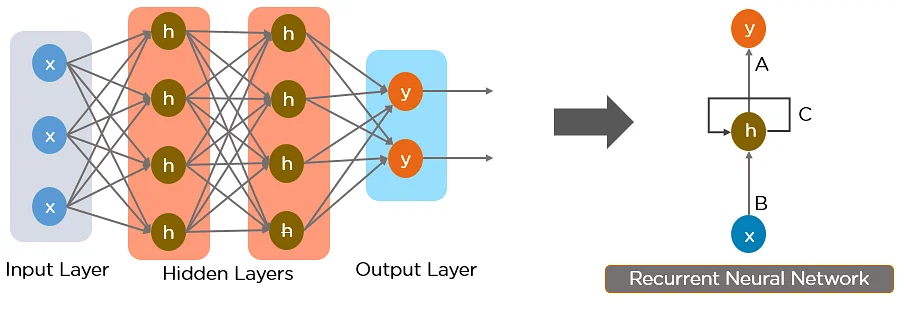
\includegraphics[width=1\linewidth]{Apendices/Figuras/modelagem-24h/8s40xcsn}
	
	\fonte{\cite{Zhang2021}}
\end{figure}

\subsubsection{Compreendendo Redes de Mem\'oria de Curto e Longo Prazo (LSTM)}

As Redes de Memória de Curto e Longo Prazo (LSTM) são uma evolução das Redes Neurais Recorrentes (RNNs), projetadas para superar desafios na captura de dependências de longo prazo em sequências de dados. Diferentemente das RNNs convencionais, as LSTMs têm a capacidade de manter informações relevantes por longos períodos, tornando-as especialmente eficazes em tarefas que envolvem padrões complexos e dependências temporais distantes.

Uma das principais inovações das LSTMs é a introdução de unidades de memória chamadas ``células'', que possuem três componentes principais: uma porta de entrada (\textit{input gate}), uma porta de esquecimento (\textit{forget gate}) e uma porta de saída (\textit{output gate}). Essas portas permitem que as LSTMs controlem o fluxo de informações através da célula, decidindo quais informações devem ser mantidas, esquecidas ou passadas para a saída.



\begin{eqnarray}
	f_t &=& \sigma(W_{xf} \cdot x_t + W_{hf} \cdot h_{t-1} + b_f) \\
	i_t &=& \sigma(W_{xi} \cdot x_t + W_{hi} \cdot h_{t-1} + b_i) \\
	\tilde{C}_t &=& \tanh(W_{xc} \cdot x_t + W_{hc} \cdot h_{t-1} + b_c) \\
	C_t &=& f_t \odot C_{t-1} + i_t \odot \tilde{C}_t \\
	o_t &=& \sigma(W_{xo} \cdot x_t + W_{ho} \cdot h_{t-1} + b_o) \\
	h_t &=& o_t \odot \tanh(C_t)
\end{eqnarray}


\noindent onde, \(x_t\) é a entrada no tempo \(t\). \(h_{t-1}\) é o estado oculto anterior no tempo \(t-1\). \(f_t\) é o valor da porta de esquecimento. \(i_t\) é o valor da porta de entrada. \(\tilde{C}_t\) é o candidato a novo estado de memória. \(C_t\) é o novo estado de memória. \(o_t\) é o valor da porta de saída. \(h_t\) é o novo estado oculto (saída) no tempo \(t\). \(\sigma\) é a função de ativação sigmoide. \(\odot\) representa a multiplicação elemento a elemento.

Essa estrutura permite que as LSTMs controlem o fluxo de informações e aprendam a armazenar ou descartar informações relevantes para diferentes tarefas. As portas de entrada, esquecimento e saída funcionam como mecanismos de controle, permitindo que as LSTMs aprendam a manter informações importantes, esquecer informações desnecessárias e gerar saídas precisas ao longo de sequências temporais.

\subsubsection{GRU (Unidade Recorrente com Port\~oes)}


Um GRU é um tipo de arquitetura de rede neural recorrente (RNN) que foi projetado para lidar com o problema de dissipação de gradiente e captura de dependências de longo prazo em sequências de dados. Essa variação das RNNs tradicionais introduz mecanismos de portão para controlar o fluxo de informação por meio das unidades de tempo.

A Gated Recurrent Unit (GRU) é uma alternativa vantajosa para a análise de séries temporais, devido à sua habilidade de lidar com sequências de dados de extensões variáveis e de capturar dependências de longo prazo presentes em informações sequenciais. Além disso, a GRU apresenta uma estrutura de simplicidade superior à LSTM, permitindo um processo de treinamento mais ágil  \cite{mastersthesis53fd58a7}.

A estrutura do GRU inclui dois portões principais: o portão de atualização (\textit{update gate}) e o portão de reinicialização (\textit{reset gate}). Esses portões permitem que o GRU decida quais informações serão transmitidas para a próxima etapa de tempo e quais informações serão descartadas.



\begin{description}
	\item[Portão de Reinicialização (\(r_t\))]: Controla a quantidade de informação do passado a ser esquecida.
	
 \begin{eqnarray}
 	r_t &=& \sigma(W_r \cdot [h_{t-1}, x_t])\label{eq:gru}
 \end{eqnarray} 

\item[Portão de Atualização (\(z_t\))]: Controla a quantidade de informação do passado a ser passada para o próximo estado.

 \begin{eqnarray}
 	z_t &=& \sigma(W_z \cdot [h_{t-1}, x_t])\label{eq:gru1}
 \end{eqnarray}

\item[Ativação do Candidato (\(h\widetilde{_t}\))]: Candidato a novo estado oculto.

\begin{eqnarray}
	h\widetilde{_t} &=& \tanh\left(W_h \cdot [r_t \odot h_{t-1}, x_t]\right)\label{eq:gru2}
\end{eqnarray}

\item[Novo Estado Oculto (\(h_t\))]: Combinação ponderada do estado anterior e do novo candidato.
\begin{eqnarray}
	h_t &=& (1 - z_t) \odot h_{t-1} + z_t \odot h\widetilde{_t}\label{eq:gru3}
\end{eqnarray}
\end{description}

\noindent nessas equações \eqref{eq:gru}, \eqref{eq:gru1}, \eqref{eq:gru2} e \eqref{eq:gru3}:
 \( h_t \) representa o estado oculto na etapa de tempo \( t \). \( h_{t-1} \) é o estado oculto na etapa de tempo anterior \( t-1 \). \( x_t \) é a entrada na etapa de tempo \( t \). \( r_t \) é o valor do portão de reinicialização na etapa \( t \). \( z_t \) é o valor do portão de atualização na etapa \( t \). \( \odot \) denota a multiplicação elemento a elemento. \( \sigma \) é a função sigmoid, que retorna valores entre 0 e 1. \( \tanh \) é a função tangente hiperbólica, que retorna valores entre $-1$ e $1$. \( W_r, W_z, W_h \) são matrizes de pesos que o modelo aprende durante o treinamento.

O GRU controla como as informações são atualizadas e propagadas ao longo do tempo, permitindo a captura de dependências de longo prazo em sequências de dados. Isso o torna uma escolha popular para tarefas que envolvem processamento de linguagem natural, como tradução automática, geração de texto, entre outras.
Na Figura \ref{fig:gru4-1024x835} tem o escama da rede neural GRU.

\begin{figure}[H]
	\centering
	\caption{Diagrama Ilustrativo do Funcionamento de uma Unidade Recorrente Gated (GRU)}
	\label{fig:gru4-1024x835}
	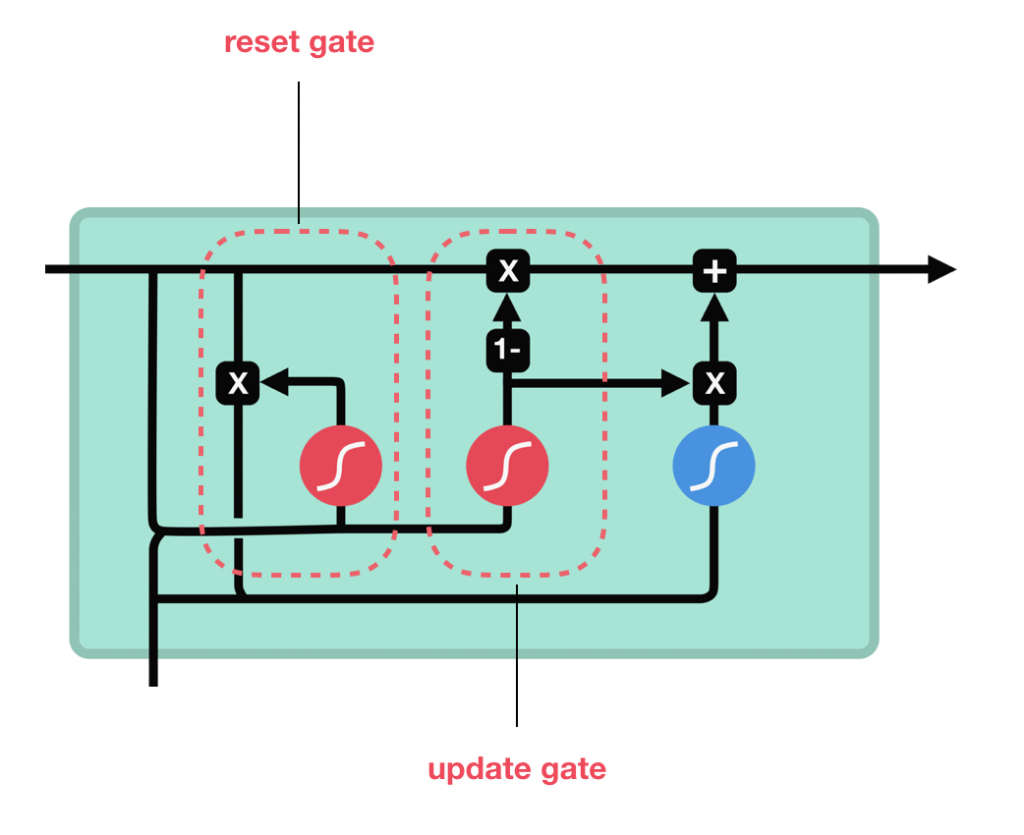
\includegraphics[width=0.5\linewidth]{Apendices/Figuras/modelagem-24h/gru4-1024x835}
	
	\fonte{\cite{DeepLearningBook2023}}
\end{figure}



\subsubsection{An\'alise Comparativa entre os Modelos RNN, LSTM e GRU}

As GRUs, as LSTMs e as RNNs são variações avançadas das arquiteturas de redes neurais, todas projetadas para abordar a dificuldade de capturar dependências temporais em sequências de dados. Cada uma dessas abordagens tem características distintas que influenciam sua capacidade de lidar com esse desafio.

Enquanto as RNNs tradicionais têm uma tendência a sofrer com o desvanecimento do gradiente ao longo do tempo, as LSTMs e GRUs foram desenvolvidas para superar essa limitação. As LSTMs introduzem células de memória e portas de controle que permitem armazenar e atualizar informações relevantes ao longo das etapas temporais, sendo especialmente adequadas para capturar relações de dependência de longo prazo. As GRUs, por sua vez, simplificam a arquitetura das LSTMs, utilizando portas de atualização e reset para permitir o fluxo de informações e controle sobre o estado oculto.

Na Figura \ref{fig:rnn-vs-lstm-vs-gru-1024x308}, há um esquema que ilustra as arquiteturas das RNNs, LSTMs e GRUs, permitindo uma visualização das diferenças entre essas abordagens.

\begin{figure}[H]
	\centering
	\caption{RNN vs LSTM vs GRU}
	\label{fig:rnn-vs-lstm-vs-gru-1024x308}
	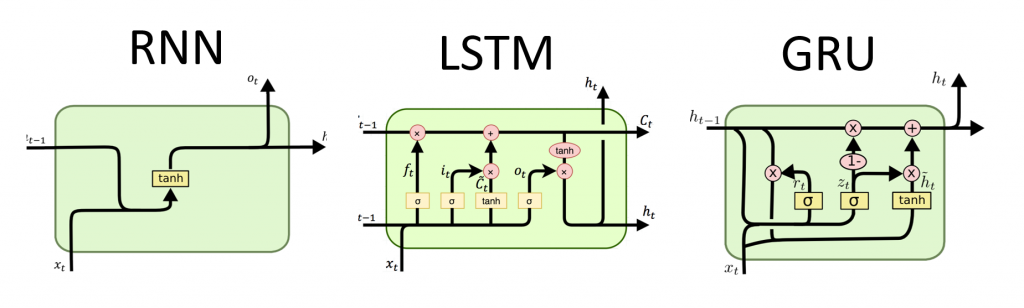
\includegraphics[width=1\linewidth]{Apendices/Figuras/modelagem-24h/RNN-vs-LSTM-vs-GRU-1024x308}
	
	\fonte{\cite{Hasan2020}}
\end{figure}


Ao observar essa imagem, é possível compreender melhor como cada uma das arquiteturas lida com a complexidade de capturar dependências temporais em sequências de dados. As LSTMs e GRUs oferecem soluções mais sofisticadas em relação às RNNs tradicionais, apresentando mecanismos que permitem capturar dependências de longo prazo de maneira mais eficaz.

\subsubsection{Explorando o Transformer: Al\'em dos Bits e Bytes}

A arquitetura de rede neural Transformer representa um avanço significativo no campo do processamento de linguagem natural e tarefas relacionadas. Foi introduzida por \cite{vaswani2017attention} e revolucionou a maneira como as redes neurais lidam com sequências de dados, superando limitações anteriores, como a dependência sequencial e a complexidade computacional. A abordagem do Transformer se destaca por sua capacidade de processar simultaneamente todas as posições de uma sequência, tornando-o altamente paralelizável e eficiente.

A equação \eqref{eq:soft} fundamental do Transformer é a autoatencão, também conhecida como mecanismo de atenção. A atenção é um conceito-chave que permite que a rede neural ``preste atenção'' a diferentes partes da entrada em graus variados, capturando relações contextuais e semânticas. A equação da autoatencão é calculada ao dividir a sequência de entrada em três representações lineares: consultas (Q), chaves (K) e valores (V). A matriz de atenção é obtida multiplicando as consultas pelas chaves transpostas e aplicando uma função de softmax aos resultados, ponderando os valores de acordo com a importância atribuída pela atenção. A saída final é uma combinação linear dos valores ponderados pela matriz de atenção.

\begin{eqnarray}
	\operatorname{Attention}(Q, K, V)=\operatorname{softmax}\left(\frac{Q K^{\mathrm{T}}}{\sqrt{d_k}}\right) V \label{eq:soft}
\end{eqnarray}

\noindent na equação \eqref{eq:soft}, embora simplificada, serve como base para a arquitetura do Transformer e é repetida várias vezes em diferentes camadas. Isso permite que a rede aprenda representações ricas e contextuais das sequências de entrada. A estrutura de múltiplas cabeças de atenção, presente no Transformer, aprimora ainda mais a capacidade da rede em capturar diferentes tipos de relações e padrões nas sequências. Em suma, o modelo Transformer revolucionou o processamento de sequências, proporcionando melhorias notáveis em tarefas como tradução automática, resumo de texto, geração de linguagem natural e muito mais. Na Figura \ref{fig:transformer} tem o esquema de como a rede neural Transformer é abordada.

\begin{figure}[H]
	\centering
	\caption{Arquitetura do Transformer}
	\label{fig:transformer}
	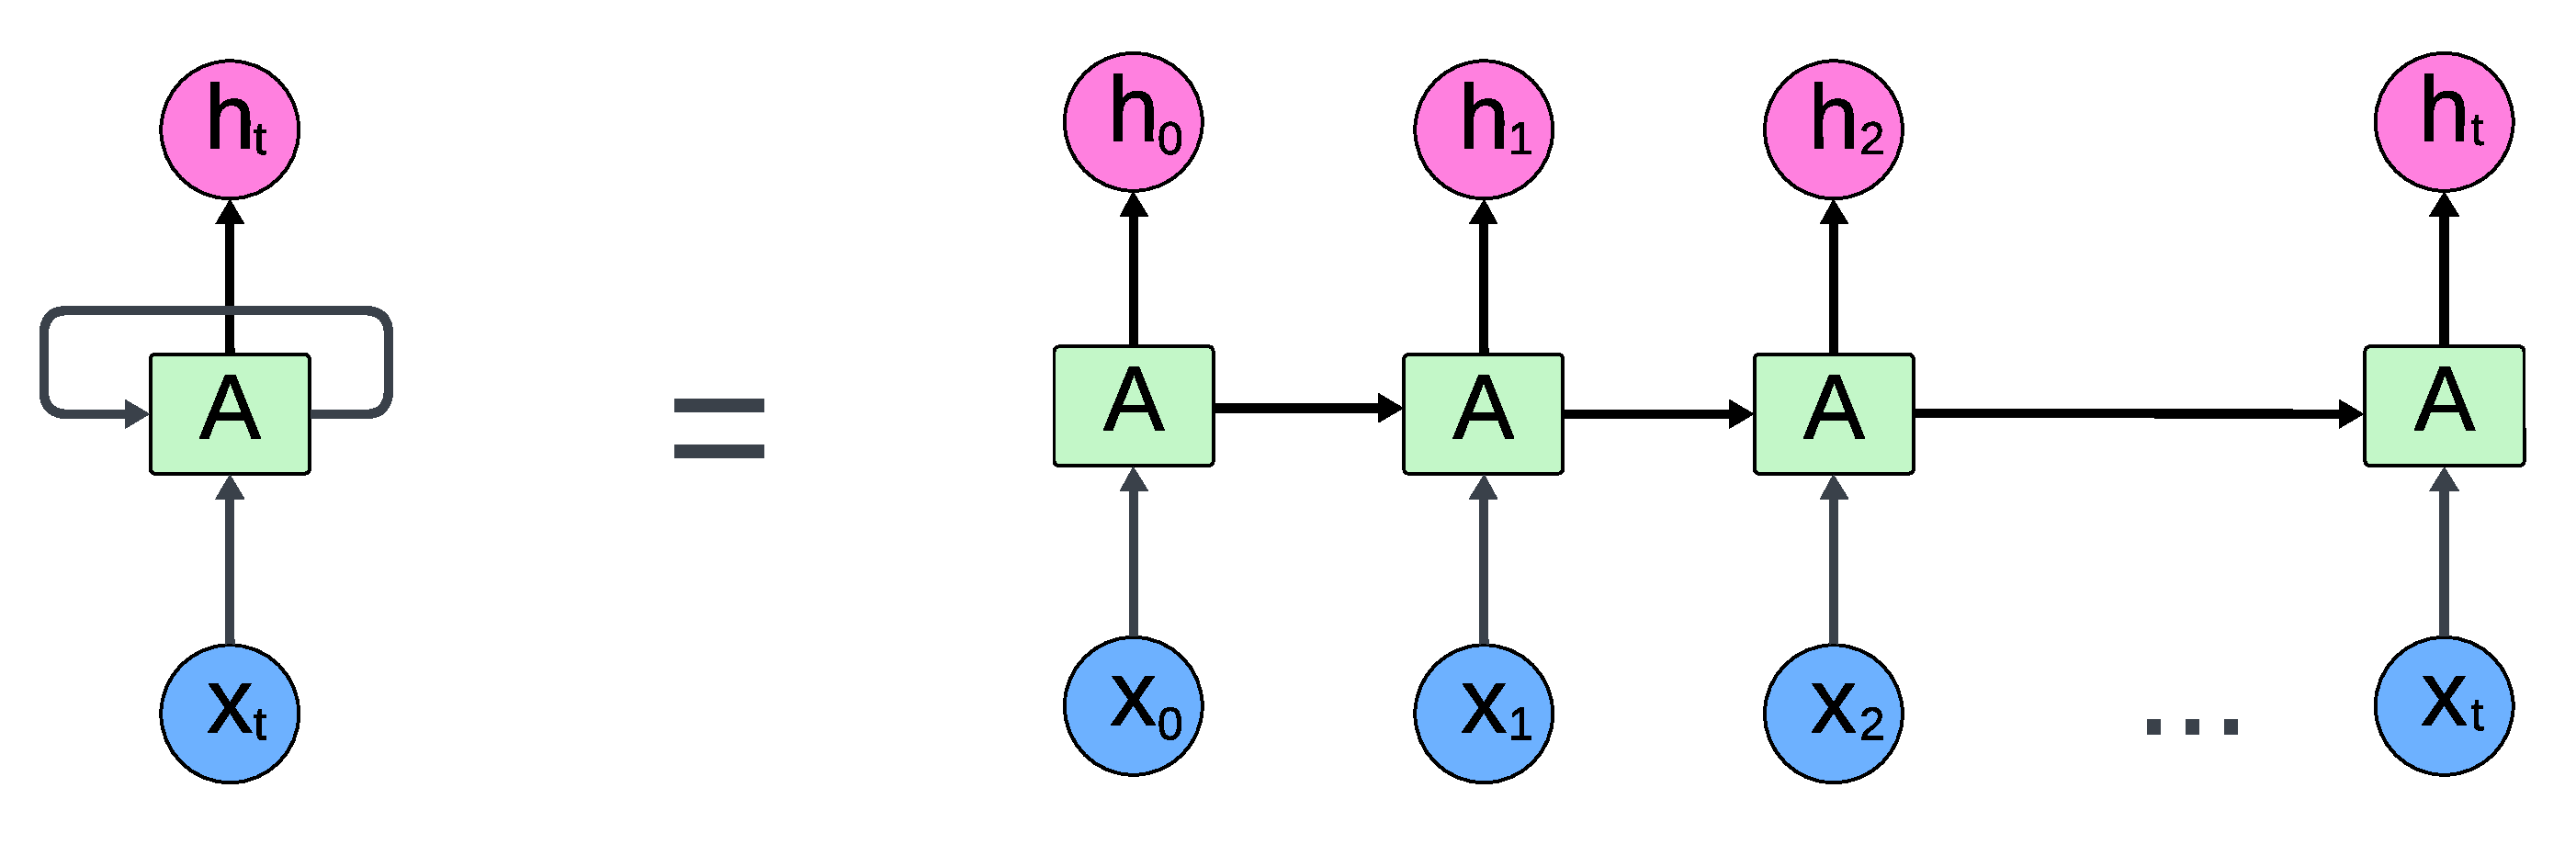
\includegraphics[width=1\linewidth]{Apendices/Figuras/modelagem-24h/Transformer}
	
	\fonte{\cite{Esposito2021}}
\end{figure}
